\documentclass[DIV=calc, paper=a4, fontsize=11pt]{scrartcl}
\usepackage{makeidx}
\usepackage{graphicx}
\usepackage{flushend}

\usepackage{lmodern}
\usepackage[left=1.5cm,right=1.5cm,top=2.5cm,bottom=2cm]{geometry}
\usepackage{float}		
\bibliographystyle{plain} 
\pagestyle{plain} 
\pagenumbering{arabic}
\usepackage{fancyhdr} 	
\usepackage[T1]{fontenc}
\usepackage[utf8]{inputenc}
\usepackage[spanish]{babel}
\usepackage[spanish,es-tabla]{babel}
\usepackage{hyperref}
\usepackage{graphicx}
\usepackage{siunitx}
\usepackage{lipsum}
\usepackage[protrusion=true,expansion=true]{microtype}
\usepackage{amsmath,amsfonts,amsthm}
\usepackage[svgnames]{xcolor}
\usepackage[svgnames]{xcolor}
\usepackage{booktabs}
\usepackage{fix-cm}
\usepackage{multicol}
\usepackage{url}
\bibliographystyle{unsrt}

\newenvironment{Figura}
  {\par\medskip\noindent\minipage{\linewidth}}
  {\endminipage\par\medskip}

\usepackage{sectsty}
\allsectionsfont{\usefont{OT1}{phv}{b}{n}}
\usepackage{fancyhdr}
\pagestyle{fancy}
\usepackage{lastpage}
\lhead{}
\chead{}
\rhead{}
\lfoot{}
\cfoot{}
\rfoot{\footnotesize Page \thepage\ of \pageref{LastPage}}
\renewcommand{\headrulewidth}{0.0pt}
\renewcommand{\footrulewidth}{0.4pt}
\usepackage{lettrine}
\newcommand{\initial}[1]{\lettrine[lines=3,lhang=0.3,nindent=0em]{
\color{DarkGoldenrod}{\textsf{#1}}}{}}
\usepackage{titling}
\newcommand{\HorRule}{\color{DarkGoldenrod} \rule{\linewidth}{1pt}}
\pretitle{\vspace{-120pt} \begin{flushleft} \HorRule \fontsize{22}{35} \usefont{OT1}{phv}{b}{n} \color{DarkRed} \selectfont}
\title{Práctica 1. \\ %Aquí va el nombre de la práctica 
Incertidumbres y análisis gráfico de mediciones} %Numero de la práctica 
\posttitle{\par
\end{flushleft}
\vskip 0.5em}
\preauthor{\begin{flushleft}\large \lineskip 0.5em \usefont{OT1}{phv}{b}{sl} \color{DarkRed}}
\author{Angel Yair García Pérez \\
Misael Iván Macías Márquez\\
Teodora Irene Ortíz Cruz\\
\small{teodora625@ciencias.unam.mx}\\}
\postauthor{\footnotesize \usefont{OT1}{phv}{m}{sl} \color{Black}
\vspace*{0.1cm} 
Facultad de Ciencias, UNAM
\par\end{flushleft}\HorRule}
\date{21 de Marzo del 2022\\Semestre 2022-2}
\begin{document}
\maketitle
\begin{abstract}
\definecolor{carmine}{rgb}{0.59, 0.0, 0.09}
 \textcolor{carmine}{\textbf{Resumen:}} Se determinó la aceleración de la gravedad local haciendo uso de un péndulo armado con material casero. Se midió con un cronómetro el tiempo de 10 oscilaciones de un péndulo simple, se aplicó el modelo clásico para el periodo de oscilación, se hizo un análisis gráfico utilizando errores nominales y estadísticos para tratar los datos obtenidos, la gravedad promedio obtenida fue $(9.36 \pm 1.54)m/s^2$ dando una incertidumbre relativa del $16\%$ y un error, comparando con un valor de referencia, de $0.27$ veces la incertidumbre absoluta, al ser menor a $2$ se puede considerar que el resultado es satisfactorio.
\end{abstract}
%%%%%%%%%%%%%%%%%%%%%%%%%%%%%%%%%%%%%%%%%%%%%%%%%%%%%%%%%%%%%%%%%%%%%%%%%%%%%%%%%%%%%%%%%%%%%%%%%%%%%%%%%%%%%%%%%%%%%%%%
\definecolor{carmine}{rgb}{0.59, 0.0, 0.09}
\section*{\textcolor{carmine}{Introducción}}
El propósito de este experimento es obtener el valor la aceleración gravitacional  $g$ en la zona metropolitana de México, utilizando la ecuación clásica para el periodo de oscilación de un péndulo simple y  aplicar la teoría de incertidumbres de manera adecuada a dicho modelo\cite{Manual}.\\
La importancia de este trabajo radica en el uso adecuado de la teoría  de incertidumbres, pues aún que es un experimento simple, el uso no adecuado de ella puede llevar a resultados desfavorables, por otro lado también se resalta la importancia del modelo empleado para medir la gravedad en este trabajo, pues fue una de la primeras formas de medir $g$ en distintas partes del mundo incluyendo México \cite{RevMexFis}.\\
De acuerdo a los experimentos realizados a partir 1878 por Francisco Jimenéz y Leadro Fernández  el valor de  $g$  es aproximadamente  $(9.7816\pm0.0001)\frac{m}{s^{2}}$ en lo que hoy en día es el Palacio Nacional\cite{RevMexFis}. Se espera obtener un valor $g$ constante parecido al que fue reportado en los estudios de Jimenéz y Fernández. 
%por lo que la hipótesis de este trabajo es que $g$ es la constante $(9.7816\pm0.0001)\frac{m}{s^{2}}$.
%, es decir, el valor de $g$ no cambia con el tiempo, 

\definecolor{carmine}{rgb}{0.59, 0.0, 0.09}
\subsection*{\textcolor{carmine}{Teoría del péndulo simple}}
Un péndulo simple se conforma de una partícula de masa $m$ suspendida de un punto $O$ por una cuerda de longitud $L$ y de masa despreciable, si la masa se lleva a un punto tal que la cuerda forme un ángulo $\theta$ con la vertical y se suelta, esta comenzará a oscilar entre el punto inicial y su simétrico respecto la vertical\cite{Finn}.
\begin{figure}[]
    \centering
    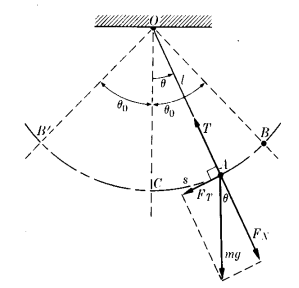
\includegraphics[width=5cm]{pendulo.PNG}
    \caption{{\textbf{Diagrama de un péndulo simple.} En este diagrama se observa un péndulo simple conformado por una masa puntual y también las fuerzas que existen en el movimiento.\cite{Finn}}}
    \label{fig:my_label}
\end{figure}
Las fuerzas que actúan sobre la partícula son el peso $mg$, la tensión $T$ y como se puede ver en la Figura 1, la fuerza tangencial $F_T = -mg \sin{\theta}$, por lo tanto la ecuación diferencial que describe este fenómeno es:
\begin{equation}
    \frac{d^2 \theta}{d t^2} + \frac{g}{L} \sin{\theta} = 0
\end{equation}
\noindent suponiendo que el ángulo $\theta$ sea lo suficientemente pequeño, es decir entre $10^{\circ}$ a $15^{\circ}$ se puede aproximar $\sin{\theta} \approx \theta$ y así se tiene que\cite{Finn}:
\begin{equation}
    \frac{d^2 \theta}{d t^2} + \frac{g}{L} \theta = 0
\end{equation}
Lo cual es muy parecido a la ecuación diferencial para el movimiento armónico simple con $\omega ^2 = \frac{g}{L}$, dado que el período en función de la frecuencia angular es $T =\frac{ 2 \pi} {\omega}$, entonces $T= \frac{2\pi} {\sqrt{\frac{g}{L}}}$, de tal forma en que despejando $g$ se obtiene la ecuación clásica para el periodo de oscilación de un péndulo simple
\begin{equation}
    g = \frac{4 \pi^2 L}{T^2}
\end{equation}
%%%%%%%%%%%%%%%%%%%%%%%%%%%%%%%%%%%%%%%%%%%%%%%%%%%%%%%%%%%%%%%%%%%%%%%%%%%%%%%%%%%%%%%%%%%%%%%%%%%%%%%%%%%%%%%

\definecolor{carmine}{rgb}{0.59, 0.0, 0.09}
\section*{\textcolor{carmine}{Desarrollo experimental}}
Como se puede observar en la Figura 2, en un soporte metálico sujetado a una repisa se introdujo una hoja de papel pegada a un pedazo de folder para mantenerla rígida, con ayuda de un transportador se marcaron los ángulos $\pm 15^{\circ}$, se ajusto el hilo cáñamo sobre el soporte y en el otro extremo del hilo se sujetó un tornillo de $76g$, su eje de simetría se coloco verticalmente para que coincidiera con la vertical del péndulo.
\begin{figure}[H]
    \centering
    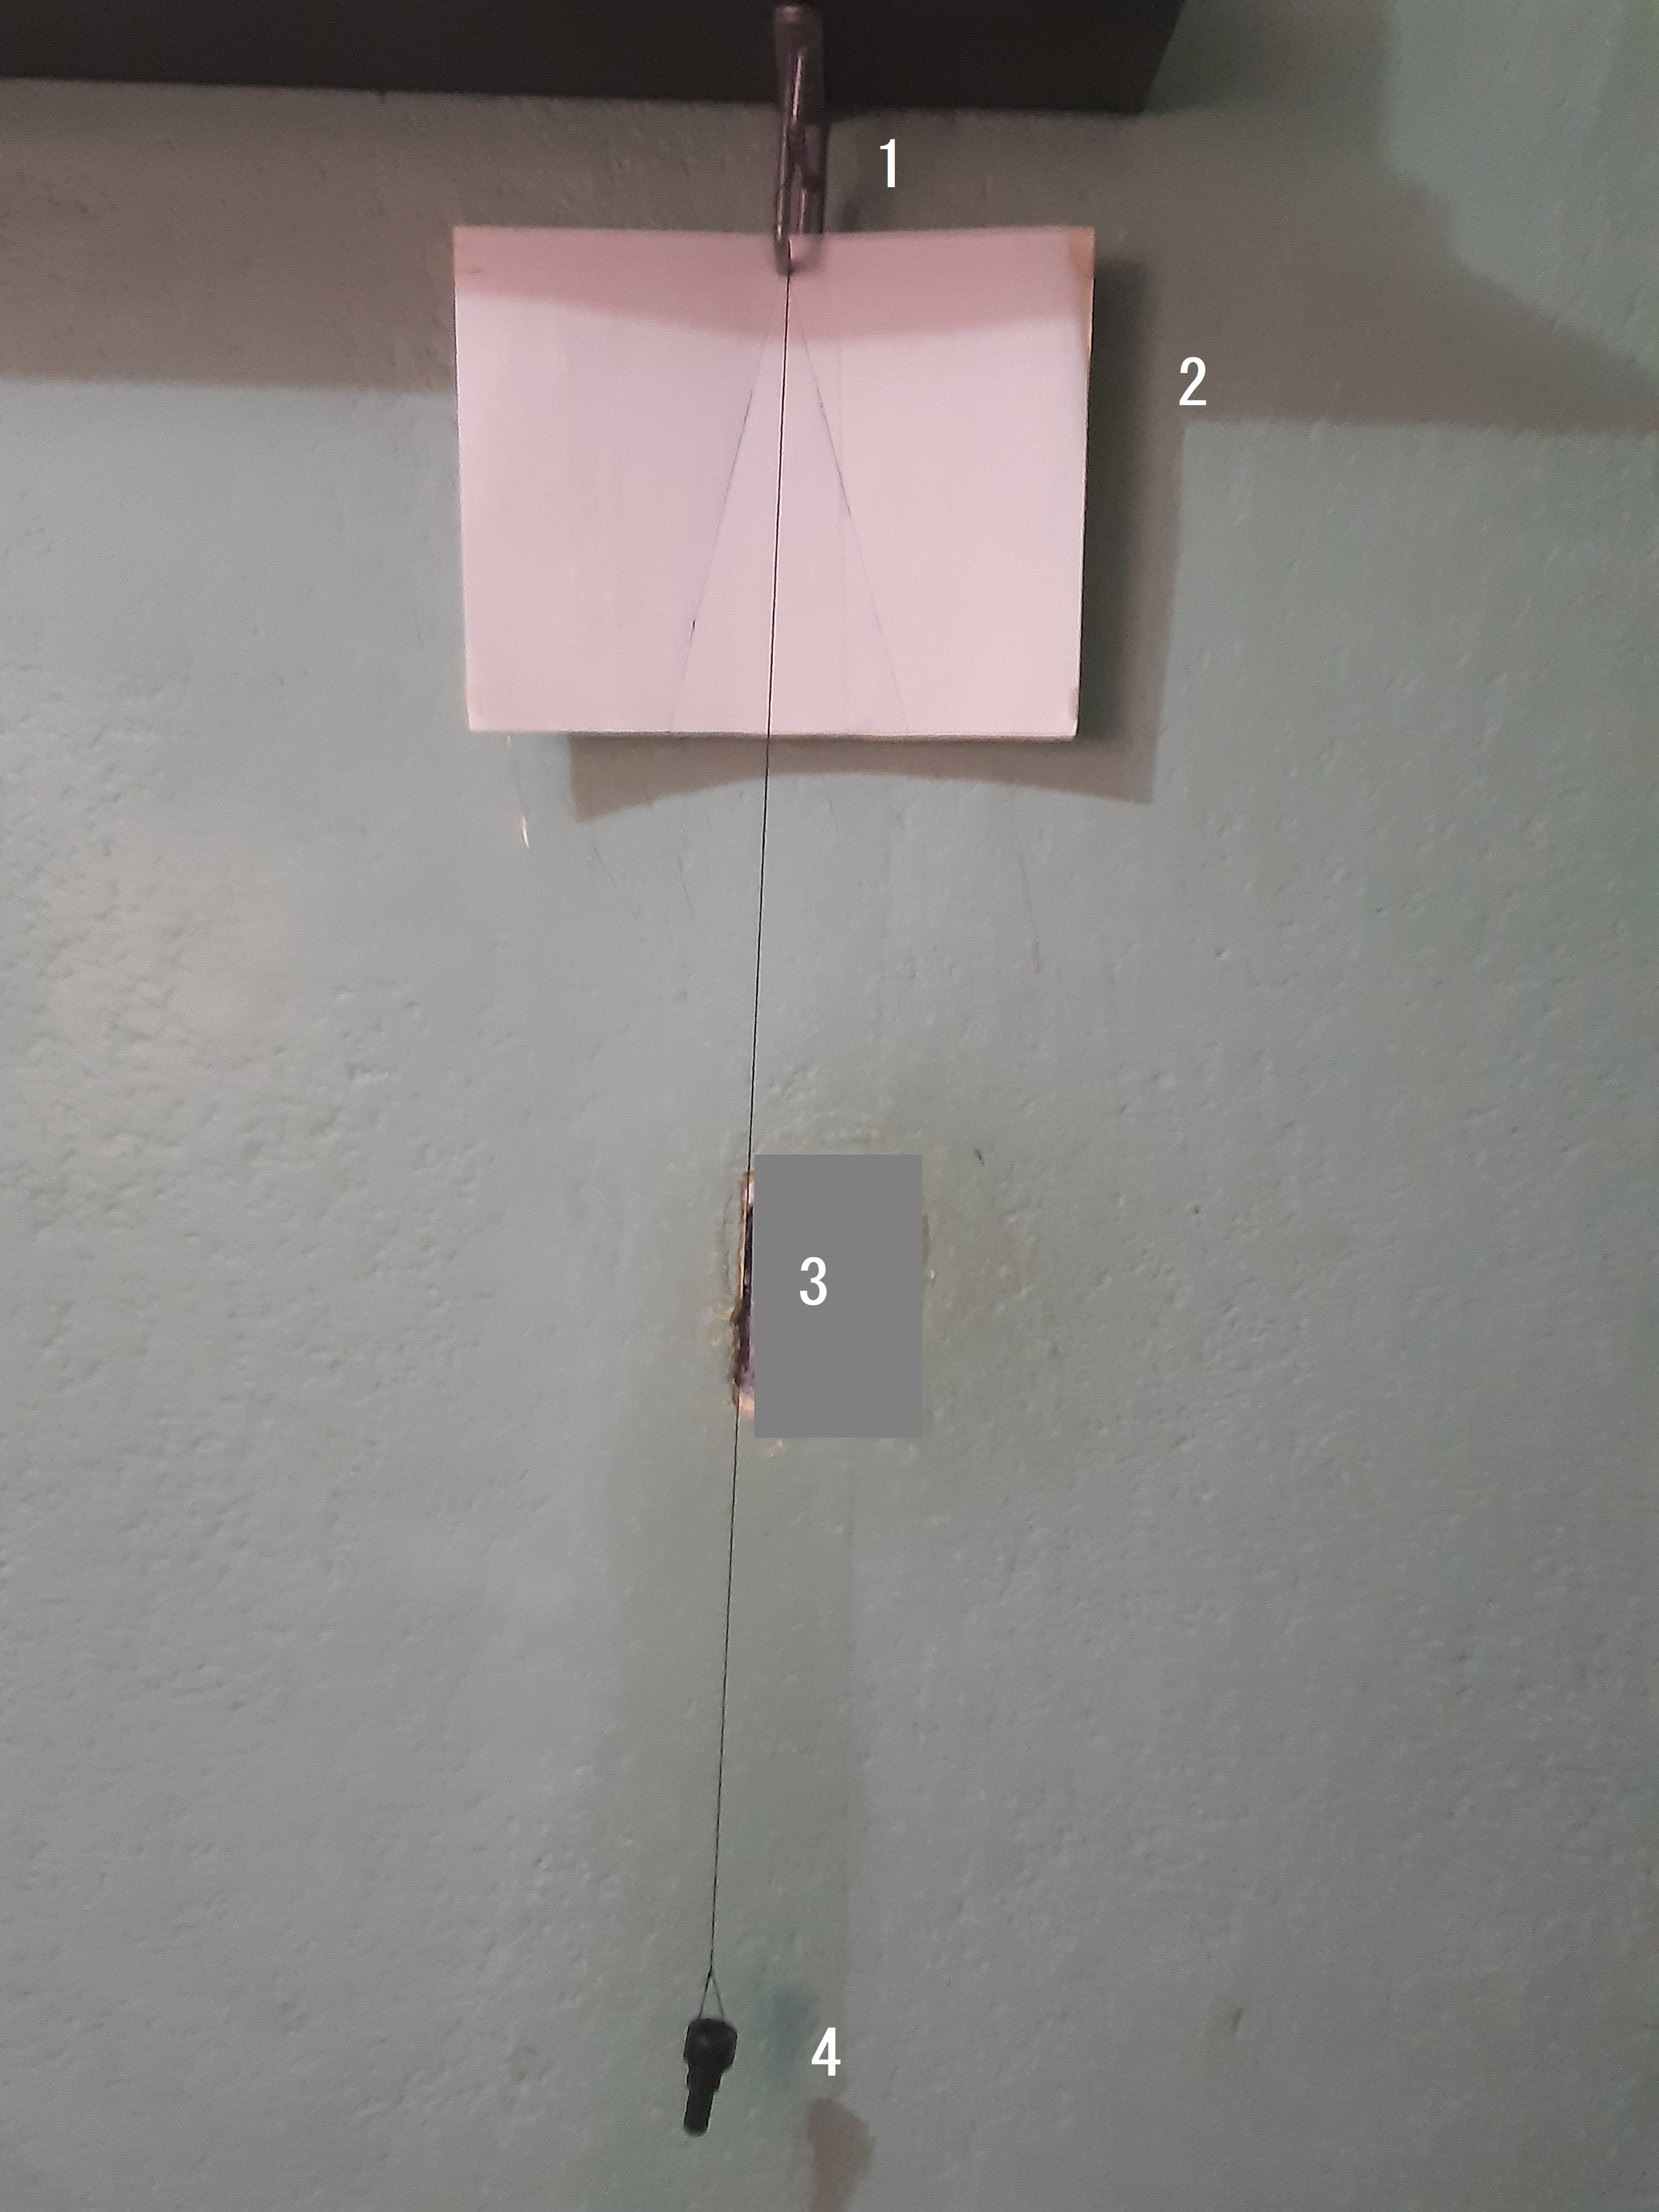
\includegraphics[width=7cm]{20220309_153216.jpg}
    \caption{\textbf{Arreglo Experimental.} Consiste en (1) Soporte de repisa,(2) Papel con marca de ángulos, (3) Hilo cáñamo, (4) Tornillo}
    \label{fig:my_label}
\end{figure}

%%%%%%%%%%%%%%%%%%%%%%%%%%%%%%%%%%%%%%%%%%%%%%%%%%%%%%%%%%%%%%%%%%%%%%%%%%%%%%%%%%%%%%%%%%%%%%%%%%%%%%%%%%%%%%%%

\subsection*{\textcolor{carmine}{Procedimiento}}
Para medir el tiempo de una oscilación, primero con una cinta métrica se midió la longitud del hilo desde su origen hasta el centro de masa del tornillo. Después se realizaron  5 medidas preliminares de tiempo para 10 oscilaciones, colocando el tornillo en el ángulo $15^{\circ}$ de lado derecho y soltándolo para dejarlo oscilar, estos tiempos se dividieron sobre 10 para hallar el tiempo de una oscilación ($T$) y se saco el promedio de las 5 medidas. El procedimiento se repitió para 10 longitudes $L$ del péndulo. 

%%%%%%%%%%%%%%%%%%%%%%%%%%%%%%%%%%%%%%%%%%%%%%%%%%%%%%%%%%%%%%%%%%%%%%%%%%%%%%%%%%%%%%%%%%%%%%%%%%%%%%%%%%%%%%%%

\section*{\textcolor{carmine}{Resultados y Análisis}}
En el experimento, para distintas longitudes, se obtuvieron los siguientes resultados:

\begin{table}[h!]
\centering
\begin{tabular}{||c|c|c||} 
 \hline
 Longitud ($L$) [$m$] & Periodo promedio ($\hat{T}$) [$s$] & gravedad ($g$) [$m/s^2$] \\ [0.5ex] 
 \hline\hline
 1 $\pm$ 0.05 & 2.024 $\pm$ 0.089  & 9.637 \\ 
 0.9 $\pm$ 0.05 &  1.928 $\pm$ 0.089 & 9.558 \\
 0.8 $\pm$ 0.05 & 1.819 $\pm$ 0.089 & 9.545 \\
 0.7 $\pm$ 0.05 &  1.703 $\pm$ 0.089 & 9.529 \\
 0.6 $\pm$ 0.05 &  1.576 $\pm$ 0.089 & 9.537 \\
 0.5 $\pm$ 0.05 & 1.440 $\pm$ 0.089 & 9.519 \\
 0.4 $\pm$ 0.05 & 1.290 $\pm$ 0.089 & 9.489 \\
 0.3 $\pm$ 0.05 & 1.127 $\pm$ 0.089 & 9.325 \\
 0.2 $\pm$ 0.05 & 0.932 $\pm$ 0.089 & 9.090 \\
 0.1 $\pm$ 0.05 & 0.686 $\pm$ 0.089 & 8.389 \\
  [1ex] 
 \hline
\end{tabular}
\caption{Valores de longitud y periodo promedio obtenidos a partir de las mediciones tomadas en el experimento, con ellos se calculo el valor de la gravedad.}
\label{table:1}
\end{table}

$\hat{T}$ se obtuvo del promedio de los $5$ periodos del apéndice para cada respectiva longitud y  $g$ fue hallada mediante la ecuación (3):
$$g=4\pi^2 \frac{L}{\hat{T}^2}$$
Sacando el promedio de la gravedad se obtuvo que:
$$\hat{g}=9.362m/s^2$$
De las medidas directas se tiene que la incertidumbre de ángulo y la masa del tornillo están dadas por la mínima escala:
\begin{equation*}
    \delta\theta =   1 ^{\circ} \hspace{1cm} \delta m =  1g
\end{equation*}
Para la longitud del péndulo se obtuvo una incertidumbre de definición $\sigma_{def, L}= \pm 5cm$,  debido a que no fue posible encontrar la localización de el centro de masa del tornillo de forma precisa, se encontró que podía estar en un rango de posiciones, además se debe resaltar que la longitud del péndulo variaba un poco mientras oscilaba porque se colgó sobre un soporte de techo redondo, sin embargo se desprecio esta incertidumbre pues era una variación pequeña, también se obtuvo una incertidumbre de apreciación  $\sigma_{ap, L}= 0.05cm$, sumando por cuadraturas se obtiene que la incertidumbre de la longitud es:

\begin{equation*}
    \delta L = \sqrt{(5cm)^2 + (0.05cm)^2} = 5cm
\end{equation*}

Para la incertidumbre del tiempo, se midió el tiempo de reacción con el cronómetro, se obtuvieron 10 datos de 10 intentos de detener el cronómetro justo a los 3 segundos de haberlo iniciado, se tomo la diferencia de los 10 datos con los 3 segundo y  el promedio como el tiempo de reacción.\\
La incertidumbre absoluta está dada por el tiempo de reacción (ver apéndice) $\sigma_{est, T} = 0.089 s$ y la escala mínima del cronómetro $\sigma_{ap, T} = 0.001s$:

\begin{equation*}
    \delta T = \sqrt{\sigma_{est}^2 + \sigma_{ap}^2} = 0.089 s
\end{equation*}

Tomando el tiempo promedio para cada péndulo y sumando por cuadraturas, se llega a que la incertidumbre de los promedios de periodos es $\delta \hat{T} = 0.089 s$.


\subsection*{ \textcolor{carmine} {Análisis de errores nominales ($\sigma_{nom}$) y estadísticos ($\sigma_{est}$) de g}}
La incertidumbre nominal para $g$ se obtiene  a partir de la ecuación (3) de la siguiente forma:
\begin{equation*}
    \sigma_{nom, g} = \sqrt{\left(\frac{\partial g}{\partial L}\right)^2 \delta L^2 + \left(\frac{\partial g}{\partial \hat{T}}\right)^2\delta \hat{T}^2} = \frac{4\pi^2}{\hat{T}^2} \sqrt{\delta L^2 + \frac{4L^2\delta \hat{T}^2}{\hat{T}^2}} 
\end{equation*}
\noindent sustituyendo la longitud $L$ del valor de $g$ más cercano a $\hat{g}$ y su correspondiente periodo promedio $\hat{T}$, tenemos que $\sigma_{nom, g}= 1.54\hspace{0.1cm}  m/s^2 $ con una gravedad $g = 9.32\hspace{0.1cm} m/s^2$.
\\\\
Y haciendo análisis estadístico a los datos de la tabla se obtuvo:


\begin{equation*}
    S_g = 0.376 m/s^2 \hspace{1cm} N_{op} = 1 \hspace{1cm} \hat{g} = 9.362m/s^2 \hspace{1cm} \sigma_{est, g} = 0.119m/s^2
\end{equation*}

%\begin{equation}
%    g = (9.36 \pm 1.54) \hspace{0.3cm} m/s^2
%\end{equation}

\subsection*{ \textcolor{carmine} {Incertidumbre estadística por análisis gráfico}}

Para determinar $g$ se linealizó la ecuación (3) de la siguiente forma:

\begin{equation}
    l = \left(\frac{g}{4\pi^2}\right) \hat{T}^2
\end{equation}

\noindent Usando el método de mínimos cuadrados \nocite{Manual} se puede determinar la pendiente :

\begin{equation*}
    \frac{g}{4 \pi^2}
\end{equation*}

Los datos de la gráfica en la Figura 3 se pueden consultar en el apéndice.



\begin{figure}[H]
    \centering
    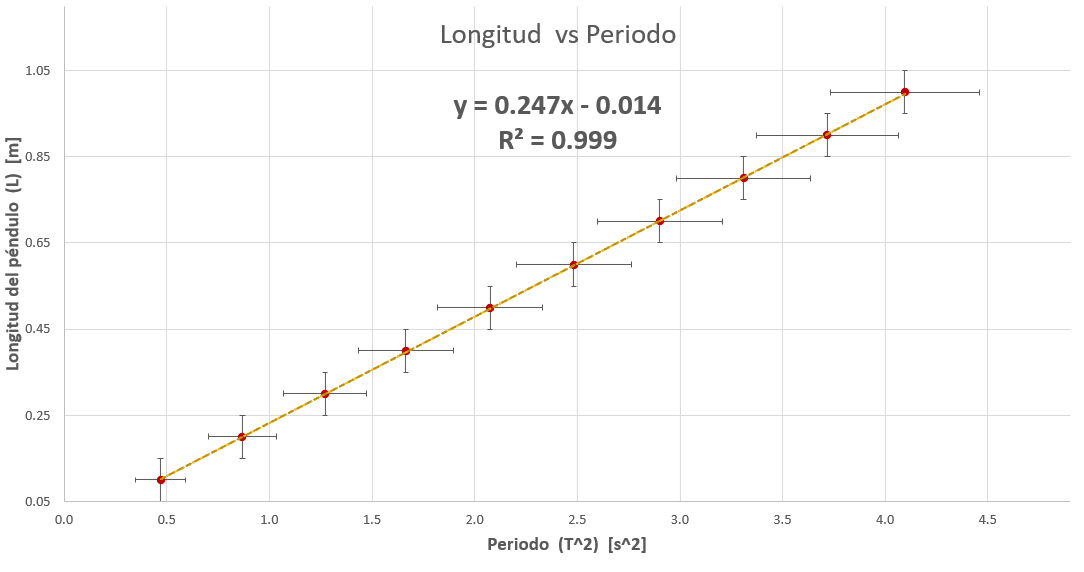
\includegraphics[width=15cm]{grafica pendulo optica.PNG}
    \caption{\textbf{Gráfica del modelo linealizado.}A partir de los datos obtenidos y el tratamiento de incertidumbres se obtuvo una gráfica donde $g$ es la pendiente, en ella se puede ver que los datos se ajustan de forma favorable al modelo lineal.}
    \label{fig:my_label}
\end{figure}

Donde la incertidumbre de $\hat{T}^2$ esta dada por:
$$\delta (\hat{T}^2)=2\hat{T}\delta T$$
La pendiente y ordenada al origen resultantes son:

\begin{equation*}
    m = (0.247 \pm 0.001) m/s^2
\end{equation*}

\begin{equation*}
    b = (0.014 \pm 0.02)\footnote{Se debe notar que el 0 entra en este intervalo} m
\end{equation*}

\noindent por lo tanto despejando a $g$ y propagando la incertidumbre,

\begin{equation*}
    g= 4\pi^2 m
\end{equation*}

\begin{equation*}
    \delta g =  4\pi^2 \delta m
\end{equation*}

\noindent se obtiene un valor para la aceleración de la gravedad de:

\begin{equation}
    g = (9.75 \pm 0.04) \hspace{0.3cm} m/s^2
\end{equation}

%sumando por cuadraturas la incertidumbre de la ecuación 5 y 6, se consigue una incertidumbre $\delta g = 1.02 \hspace{0.3cm} m/s^2$ y promediando las gravedades resultantes se tiene:

%\begin{equation}
%    g = (9.55 \pm 1.02) \hspace{0.3cm} m/s^2
%\end{equation}




\section*{\textcolor{carmine}{Discusión}}
Se observa que, en la tabla, cada vez que la longitud se hacía mas pequeña, el valor obtenido de $g$ era también mas pequeño, esto porque se hacia mas difícil detener el cronometro en el momento indicado debido a que el péndulo se movía mas rápido, parece que hubo un error sistemático.
\\
Ahora, para mediciones únicas, se utilizaría el valor de $g$ promedio con la incertidumbre $\sigma_{nom, g}$:
$$\hat{g}=(9.36\pm 1.54) m/s^2$$
Para mediciones estadísticas se utilizaría a $g$ promedio con la incertidumbre $\sigma_{est, g}$:
$$\hat{g}=(9.36\pm 0.1) m/s^2$$
O para un análisis gráfico:
\begin{equation}
    g = (9.75 \pm 0.04) \hspace{0.3cm} m/s^2
\end{equation}

\definecolor{carmine}{rgb}{0.59, 0.0, 0.09}
\section*{\textcolor{carmine}{Conclusiones}}


%El arreglo experimental usado aunque mostró algunas dificultades, considero fue suficiente para tener una buena medida de la aceleración de la gravedad ya que el error del valor real y la medición fue de $0.23 m/s^2$ o $0.23$ veces la incertidumbre absoluta de $g$ obtenida, además de tener una incertidumbre relativa de $10.4\%$, por lo tanto el resultado es satisfactorio.
Se uso un arreglo experimental casero, por lo tanto los instrumentos utilizados no fueron muy precisos ni fueron los mejores para la realización de este experimento, debido a esto la incertidumbre para las mediciones únicas fue alta, se obtuvo un error porcentual del $16\%$, esto solo da un posible rango de valores donde puede estar el valor de la gravedad, comparando con el valor de referencia $(9.7816\pm0.0001)m/s^2$ se observa que el rango de valores obtenido $[(9.36-1.54) m/s^2,(9.36+1.54)m/s^2]=[7.82m/s^2,10.9m/s^2]$ o $\hat{g}=(9.36\pm 1.54) m/s^2$ es aceptable.
\\\\
Si se compara el resultado estadístico con el valor de referencia, se puede notar que no concuerdan los resultados, por lo tanto del resultado estadístico obtenido no se puede concluir nada, se necesitaría mejorar el experimento.
\\\\
Por otro lado, el análisis gráfico dio un buen resultado, el cual concuerda con nuestro valor de referencia.
\\\\
Esto da a pensar que hubo un error sistemático al momento de tomar los datos, el cual arrastro hacia abajo el valor de $g$ , pero al parecer la tendencia se mantuvo, por lo que el análisis gráfico arrojo un buen valor.
\\\\
Al final se obtuvo un rango de valores $[7.82m/s^2,10.9m/s^2]$ donde podría estar el valor de la gravedad.
\\\\
Y un resultado estadístico para $g$:
$$g = (9.75 \pm 0.04) \hspace{0.3cm} m/s^2$$

\nocite{*}

\bibliography{biblio}

\section*{\textcolor{carmine}{Apéndice}}
\begin{multicols}
\centering

\subsection*{\textcolor{carmine}{Tiempos de reacción}}

\begin{tabular}{||c| c||} 
 \hline
 tiempo de reacción [s] & diferencia  [s] \\ [0.5ex] 
 \hline\hline
 3.010 & 0.010  \\ 
 3.021 &  0.021 \\
 2.770 & 0.230 \\
 3.094 &  0.094\\
 2.825 &  0.175\\
 2.976 & 0.024\\
 3.118 & 0.118\\
 3.103 & 0.103\\
 2.905 & 0.095\\
 3.024 & 0.024\\
  [1ex] 
 \hline
\end{tabular}
\caption{\textbf{Tabla 2:} Tiempos de reacción y su diferencia con $3s$}

\begin{equation*}
    \hat{x} = 0.089s \hspace{0.3cm} S_x = 0.073 \hspace{0.3cm} \sigma_{est} = 0.023 \hspace{0.3cm} \sigma_{ap} = 0.01s
\end{equation*}

$\vspace{-1.5cm}$

\begin{equation*}
     \hspace{0.3cm} N_{op} = 54
\end{equation*}

\subsection*{\textcolor{carmine}{Tiempos medidos}}

\begin{tabular}{||c| c||} 
 \hline
 tiempo (t) $\pm$ 0.089 [s] & período (T) \pm 0.089 [s] \\ [0.5ex] 
 10 oscilaciones &  \\
 \hline\hline
 20.209 & 2.021  \\ 
 20.221 & 2.022  \\
 20.214 & 2.021 \\
 20.297 & 2.030 \\
 20.239 & 2.024 \\
  [1ex] 
 \hline
\end{tabular}

\caption{\textbf{Tabla 3:} Datos del péndulo con longitud de $(1 \pm 0.05)m$ }

\begin{equation*}
    \hat{T} = 2.024s \hspace{0.3cm} S_T= 0.004s \hspace{0.3cm} \sigma_{est} = 0.002s \hspace{0.3cm} \sigma_{ap} = 0.001s 
\end{equation*}

$\vspace{-1.5cm}$

\begin{equation*}
    N_{op} = 1
\end{equation*}


\begin{tabular}{||c| c||} 
 \hline
 tiempo (t) \pm 0.089 [s] & período (T) \pm 0.089 [s] \\ [0.5ex] 
 10 oscilaciones &  \\
 \hline\hline
 19.278 & 1.928  \\ 
 19.198 & 1.920  \\
 19.273 & 1.927 \\
 19.317 & 1.932 \\
 19.347 & 1.935 \\
  [1ex] 
 \hline
\end{tabular}

\caption{\textbf{Tabla 4:}Datos del péndulo con longitud de $(0.9 \pm 0.05 )m$}

\begin{equation*}
    \hat{T} = 1.928s \hspace{0.3cm} S_T= 0.006s \hspace{0.3cm} \sigma_{est} = 0.003s \hspace{0.3cm} \sigma_{ap} = 0.001s 
\end{equation*}

$\vspace{-1.5cm}$

\begin{equation*}
    N_{op} = 1
\end{equation*}




\begin{tabular}{||c| c||} 
 \hline
 tiempo (t) \pm 0.089 [s] & período (T) \pm 0.089 [s] \\ [0.5ex] 
 10 oscilaciones &  \\
 \hline\hline
 18.181 & 1.808  \\ 
 18.225 & 1.823  \\
 18.120 & 1.812 \\
 18.234 & 1.823 \\
 18.204 & 1.820 \\
  [1ex] 
 \hline
\end{tabular}

\caption{\textbf{Tabla 5:} Datos del péndulo con longitud de $(0.8 \pm 0.05)m$}

\begin{equation*}
    \hat{T} = 1.819s \hspace{0.3cm}S_T= 0.005s \hspace{0.3cm} \sigma_{est} = 0.002s \hspace{0.3cm} \sigma_{ap} = 0.001s 
\end{equation*}

$\vspace{-1.5cm}$

\begin{equation*}
    N_{op} = 1
\end{equation*}


\begin{tabular}{||c| c||} 
 \hline
 tiempo (t) \pm 0.089 [s] & período (T) \pm 0.089 [s] \\ [0.5ex] 
 10 oscilaciones &  \\
 \hline\hline
 17.096 & 1.710  \\ 
 17.044 & 1.704  \\
 16.963 & 1.696 \\
 17.060 & 1.706 \\
 17.010 & 1.701 \\
  [1ex] 
 \hline
\end{tabular}

\caption{\textbf{Tabla 6:}Datos del péndulo con longitud de $(0.7 \pm 0.05)m$}

\begin{equation*}
    \hat{T} = 1.703s \hspace{0.3cm}S_T= 0.005s \hspace{0.3cm} \sigma_{est} = 0.002s \hspace{0.3cm} \sigma_{ap} = 0.001s 
\end{equation*}

$\vspace{-1.5cm}$

\begin{equation*}
    N_{op} = 1
\end{equation*}


\begin{tabular}{||c| c||} 
 \hline
 tiempo (t) \pm 0.089 [s] & período (T) \pm 0.089 [s] \\ [0.5ex] 
 10 oscilaciones &  \\
 \hline\hline
 15.748 & 1.575  \\ 
 15.725 & 1.573  \\
 15.780 & 1.578 \\
 15.802 & 1.580 \\
 15.739 & 1.574 \\
  [1ex] 
 \hline
\end{tabular}

\caption{\textbf{Tabla 7:} Datos del péndulo con longitud de $(0.6 \pm 0.05)m$}

\begin{equation*}
    \hat{T} = 1.576s \hspace{0.3cm}S_T= 0.003s \hspace{0.3cm} \sigma_{est} = 0.001s \hspace{0.3cm} \sigma_{ap} = 0.001s 
\end{equation*}

$\vspace{-1.4cm}$

\begin{equation*}
    N_{op} = 1
\end{equation*}



\begin{tabular}{||c| c||} 
 \hline
 tiempo (t) \pm 0.089 [s] & período (T) \pm 0.089 [s] \\ [0.5ex] 
 10 oscilaciones &  \\
 \hline\hline
 14.359 & 1.436  \\ 
 14.437 & 1.444  \\
 14.404 & 1.440 \\
 14.453 & 1.445 \\
 14.362 & 1.436 \\
  [1ex] 
 \hline
\end{tabular}
\caption{\textbf{Tabla 8:} Datos del péndulo con longitud de $(0.5\pm 0.05 )m$}

\begin{equation*}
    \hat{T} = 1.440s \hspace{0.3cm} S_T= 0.004s \hspace{0.3cm} \sigma_{est} = 0.002s \hspace{0.3cm} \sigma_{ap} = 0.001s 
\end{equation*}

$\vspace{-1.5cm}$

\begin{equation*}
    N_{op} = 1
\end{equation*}



\begin{tabular}{||c| c||} 
 \hline
 tiempo (t) \pm 0.089 [s] & período (T) \pm 0.089 [s] \\ [0.5ex] 
 10 oscilaciones &  \\
 \hline\hline
 12.893 & 1.289  \\ 
 12.951 & 1.295  \\
 12.964 & 1.296 \\
 12.854 & 1.285 \\
 12.836 & 1.284 \\
  [1ex] 
 \hline
\end{tabular}

\caption{\textbf{Tabla 9:} Datos del péndulo con longitud de $(0.4\pm 0.05) m$}

\begin{equation*}
    \hat{T} = 1.290s \hspace{0.3cm} S_T= 0.006s \hspace{0.3cm} \sigma_{est} = 0.003s \hspace{0.3cm} \sigma_{ap} = 0.001s 
\end{equation*}
$\vspace{-1.5cm}$

\begin{equation*}
    N_{op} = 1
\end{equation*}

\begin{tabular}{||c| c||} 
 \hline
 tiempo (t) \pm 0.089 [s] & período (T) \pm 0.089 [s] \\ [0.5ex] 
 10 oscilaciones &  \\
 \hline\hline
 11.294 & 1.129  \\ 
 11.281 & 1.128  \\
 11.241 & 1.124 \\
 11.247 & 1.125 \\
 11.305 & 1.131 \\
  [1ex] 
 \hline
\end{tabular}
\caption{\textbf{Tabla 10:} Datos del péndulo con longitud de $(0.3\pm 0.055) m$}


\begin{equation*}
   \hat{T} = 1.127s \hspace{0.3cm} S_T= 0.003s \hspace{0.3cm} \sigma_{est} = 0.001s \hspace{0.3cm} \sigma_{ap} = 0.001s 
\end{equation*}

$\vspace{-1.5cm}$

\begin{equation*}
    N_{op} = 1
\end{equation*}



\begin{tabular}{||c| c||} 
 \hline
 tiempo (t) \pm 0.089 [s] & período (T) \pm 0.089 [s] \\ [0.5ex] 
 10 oscilaciones &  \\
 \hline\hline
 9.263 & 0.926  \\ 
 9.316 & 0.932  \\
 9.363 & 0.936 \\
 9.314 & 0.931 \\
 9.331 & 0.933 \\
  [1ex] 
 \hline
\end{tabular}

\caption{\textbf{Tabla 11:} Datos del péndulo con longitud de $(0.2\pm 0.05 )m$}

\begin{equation*}
    \hat{T} = 0.932s \hspace{0.3cm} S_T= 0.004s \hspace{0.3cm} \sigma_{est} = 0.002s \hspace{0.3cm} \sigma_{ap} = 0.001s 
\end{equation*}

$\vspace{-1.5cm}$

\begin{equation*}
    N_{op} = 1
\end{equation*}



\begin{tabular}{||c| c||} 
 \hline
 tiempo (t) \pm 0.089 [s] & período (T) \pm 0.089 [s] \\ [0.5ex] 
 10 oscilaciones &  \\
 \hline\hline
 6.775 & 0.677  \\ 
 6.811 & 0.681  \\
 6.887 & 0.689 \\
 6.899 & 0.690 \\
 6.913 & 0.691 \\
  [1ex] 
 \hline
\end{tabular}

\caption{\textbf{Tabla 12:} Datos del péndulo con longitud de $(0.1\pm 0.05) m$}

\begin{equation*}
    \hat{T} = 0.686s \hspace{0.3cm} S_T= 0.006s \hspace{0.3cm} \sigma_{est} = 0.003s \hspace{0.3cm} \sigma_{ap} = 0.001s 
\end{equation*}

$\vspace{-1.5cm}$

\begin{equation*}
    N_{op} = 1
\end{equation*}

\end{multicols}
\end{document}
\end{document}
